% ============================================================
%  Apresentação — Banca PFC I
%  Avaliação Experimental de Heurísticas para o PSP
%  Vinicius Alves Pereira — CEFET-MG Divinópolis — 2026
% ============================================================
\documentclass{beamer}

% ---------- Tema e cores ----------
\usetheme{Darmstadt}
\usecolortheme{orchid}
\usefonttheme[onlylarge]{structurebold}
\setbeamerfont*{frametitle}{size=\normalsize,series=\bfseries}

% ---------- Idioma e codificação ----------
\usepackage[utf8]{inputenc}
\usepackage[T1]{fontenc}
\usepackage[portuguese]{babel}

% ---------- Pacotes adicionais ----------
\usepackage{graphicx}
\usepackage{times}
\usepackage{tikz}
\usetikzlibrary{arrows,shapes,positioning,calc}
\usepackage{ragged2e}
\usepackage{booktabs}
\usepackage{colortbl}
\usepackage{array}
\usepackage{amsmath}
\usepackage{amssymb}

% ---------- Sem ícones de navegação ----------
\setbeamertemplate{navigation symbols}{}

% ---------- Rodapé ----------
\setbeamertemplate{footline}{
  \leavevmode
  \begin{beamercolorbox}[wd=\paperwidth,ht=0.3cm,dp=0.2cm,
      leftskip=0.5cm,rightskip=0.5cm]{author in head/foot}
    \hbox to \paperwidth{%
      \scriptsize Vinicius Alves Pereira \quad|\quad
      PFC I — CEFET-MG Divinópolis \hfill
      Slide \insertframenumber{} de \inserttotalframenumber%
      \hspace{0.4cm}
    }%
  \end{beamercolorbox}
}

% ---------- Cores auxiliares ----------
\definecolor{destaque}{RGB}{180,0,0}
\definecolor{verde}{RGB}{0,130,60}
\definecolor{cinza}{RGB}{200,200,200}

% ---------- Metadados ----------
\title[Heurísticas para o PSP]{%
  Avaliação Experimental de Heurísticas e Meta-Heurísticas para o Problema Fracionário de Seleção de Pedidos Ótima
}
% \subtitle{Projeto Final de Curso I — Banca de Avaliação}
\author[Vinicius A.\ Pereira]{%
  Vinicius Alves Pereira \\
  \medskip
  \small{Orientador: Prof.\ Ms.\ Eduardo Gabriel Reis Miranda} \\
  \small{Coorientador: Prof.\ Dr.\ André Luiz Maravilha Silva}}
\institute{Centro Federal de Educação Tecnológica de Minas Gerais \\ Campus Divinópolis}
\date{2026}

% ============================================================
\begin{document}
% ============================================================

% ---- Capa ----
\begin{frame}[plain]
    \titlepage
\end{frame}

% ---- Sumário ----
\begin{frame}{Roteiro}
    \tableofcontents
\end{frame}

% ============================================================
\section{Introdução}
% ============================================================

\begin{frame}{E-commerce e Cadeias de Suprimentos}
    \begin{center}
        \begin{figure}
            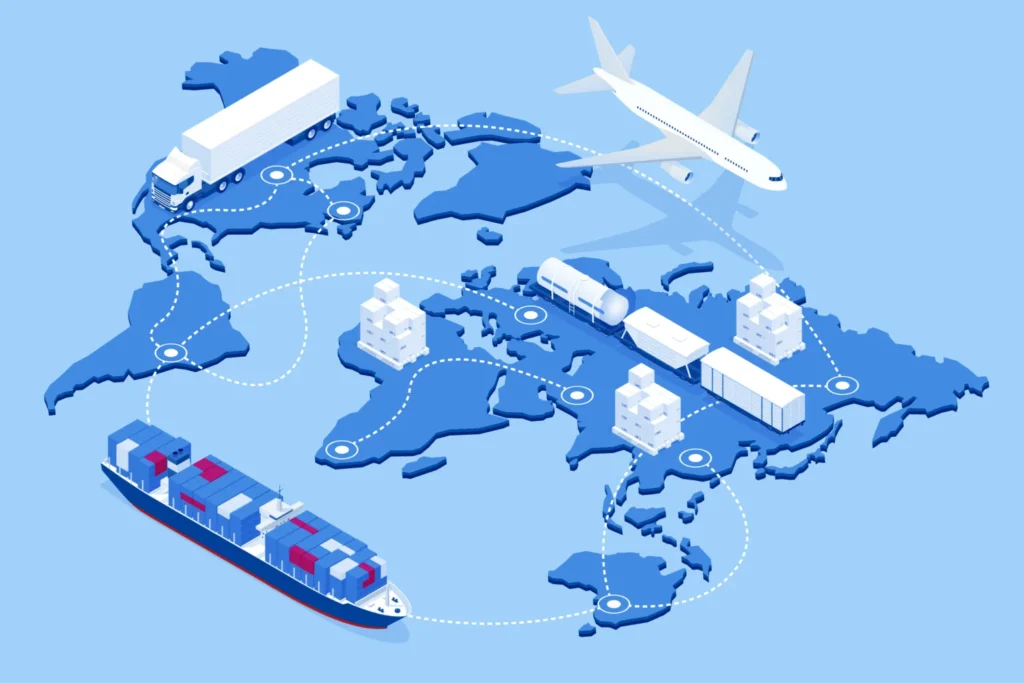
\includegraphics[width=0.8\textwidth]{Fig/supply_chain.png}
            \caption{Ilustração Cadeia de suprimentos.}
        \end{figure}
    \end{center}
\end{frame}

\begin{frame}{Armazenagem e Separação de Pedidos}
    \begin{center}
        \begin{figure}
            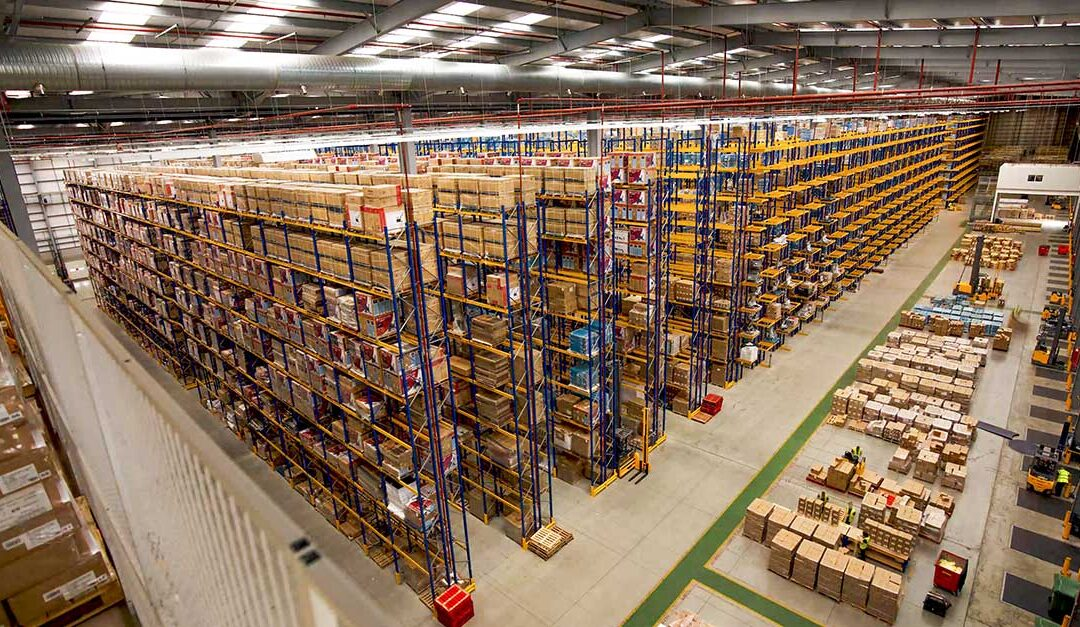
\includegraphics[width=0.8\textwidth]{Fig/warehouse.jpg}
            \caption{Exemplo de Armazém.}
        \end{figure}
    \end{center}
\end{frame}

\begin{frame}{SBPO 25}
    \begin{center}
        \begin{figure}
            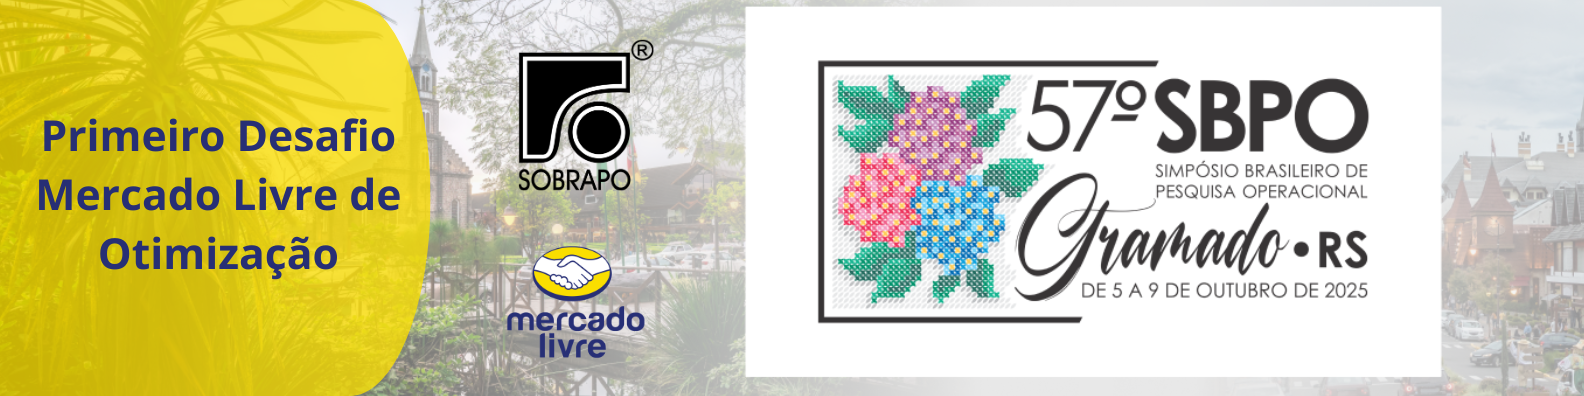
\includegraphics[width=\textwidth]{Fig/sbpo.png}
            \caption{Ilustração SBPO 25.}
        \end{figure}
    \end{center}
\end{frame}

\begin{frame}{Objetivos}
    \small
    \begin{block}{Objetivo Geral}
        Implementar e avaliar experimentalmente abordagens heurísticas para o
        \textbf{Problema de Seleção de Pedidos Ótima (PSP)}, utilizando as
        instâncias do Desafio SBPO 2025.
    \end{block}

    \bigskip
    \textbf{Objetivos Específicos:}
    \begin{enumerate}
        \item Revisão da literatura do OBP
        \item Implementar heurística gulosa
        \item Conduzir experimentos computacionais
        \item Estuar o compromisso qualidade $\times$ tempo via Fronteira de Pareto
    \end{enumerate}
\end{frame}

\begin{frame}{Literatura do OBP — Contexto e Lacuna}
    \begin{center}
        \begin{tabular}{lcc}
            \toprule
            \textbf{Método}  & \textbf{Aras (2022)} & \textbf{Pardo (2024)} \\
            \midrule
            Meta-heurísticas & 51\%                 & 61{,}6\%              \\
            Heurísticas      & 18\%                 & 36{,}8\%              \\
            Métodos Exatos   & 17\%                 & 27{,}2\%              \\
            \bottomrule
        \end{tabular}
    \end{center}
    \smallskip

\end{frame}

% ============================================================
\section{Referencial Teórico}
% ============================================================

\begin{frame}{Otimização — Quatro Elementos do Modelo}
    \small
    \begin{columns}
        \begin{column}{0.48\textwidth}
            \begin{block}{1. Variáveis de Decisão}
                Grandezas sob controle do decisor.
            \end{block}
            \vspace{0.5cm}
            \begin{block}{3. Função Objetivo}
                Critério a ser maximizado ou minimizado.
            \end{block}
        \end{column}
        \begin{column}{0.48\textwidth}
            \begin{block}{2. Constantes / Parâmetros}
                Dados conhecidos \emph{a priori}.
            \end{block}
            \vspace{0.5cm}
            \begin{block}{4. Restrições}
                Condições que delimitam as soluções viáveis.
            \end{block}
        \end{column}
    \end{columns}

    \vspace{0.8cm}
    \begin{alertblock}{}
        Modelos complexos de otimização frequentemente geram problemas \textbf{NP-difíceis}.
        Essa limitação computacional motiva o uso de métodos aproximados, como as
        \textbf{heurísticas e meta-heurísticas}.
    \end{alertblock}
\end{frame}

\begin{frame}{Heurísticas Construtivas}
    \small
    \begin{block}{O que são?}
        Procedimentos aproximados que obtêm soluções de boa qualidade em
        tempo reduzido, \textbf{sem garantia de otimalidade}.
    \end{block}

    \bigskip
    \textbf{Características:}
    \begin{itemize}
        \item Constroem a solução em \emph{uma única passagem}
        \item Decisões locais guiadas por critério guloso
        \item Sem revisão das escolhas já feitas
        \item[$\Rightarrow$] Rápidas, porém limitadas em qualidade
    \end{itemize}
\end{frame}

\begin{frame}{Meta-heurísticas}
    \small
    \begin{block}{O que são?}
        Métodos que utilizam estratégias capazes de \textbf{escapar de ótimos locais} e explorar robustamente o espaço de soluções.
    \end{block}

    \bigskip
    \begin{columns}
        \begin{column}{0.50\textwidth}
            \textbf{Conceitos centrais:}
            \begin{itemize}
                \item Representação da solução
                \item Vizinhança e movimento
                \item Busca local e ótimo local
                      \newline
                      \newline
                      \newline
            \end{itemize}
        \end{column}
        \begin{column}{0.46\textwidth}
            \textbf{Exemplos:}
            \begin{itemize}
                \item Busca Tabu
                \item GRASP
                \item Simulated Annealing
                \item Algoritmos Genéticos
                \item Colônia de Formigas
            \end{itemize}
        \end{column}
    \end{columns}

\end{frame}

\begin{frame}{Fronteira de Pareto}
    \begin{center}
        \begin{figure}
            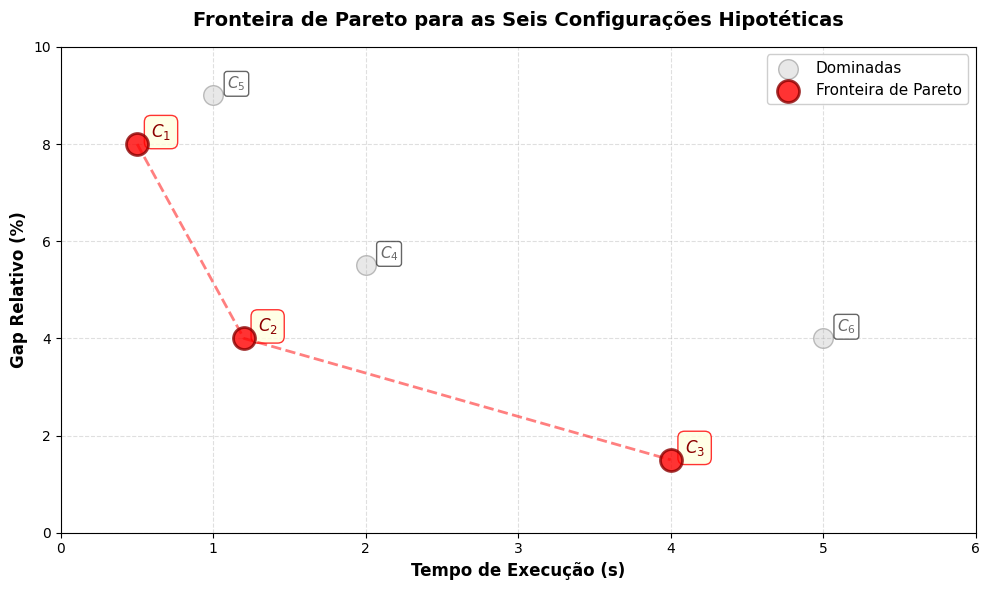
\includegraphics[width=0.75\textwidth]{Fig/exemplo_pareto.png}
            \caption{Exemplo de Fronteira de Pareto.}
        \end{figure}
    \end{center}
    \vspace{-0.3cm}
    \small
    \begin{itemize}
        \item $C_1$, $C_2$, $C_3$ — \textbf{não dominados} (Fronteira de Pareto)
        \item $C_4$ e $C_5$ — dominados; a curva tracejada delimita a fronteira
    \end{itemize}
\end{frame}

% ============================================================
\section{Definição do Problema}
% ============================================================

\begin{frame}{O Problema de Seleção de Pedidos Ótima (PSP)}
    \small
    \textbf{Dados:} backlog de pedidos, estoque nos corredores,
    limites $[\mathrm{LB}, \mathrm{UB}]$

    \bigskip
    \textbf{Decidir simultaneamente:}
    \begin{enumerate}
        \item Subconjunto de pedidos $\mathcal{O}' \subseteq \mathcal{O}$
              que compõe a \textit{wave}
        \item Subconjunto de corredores $\mathcal{A}' \subseteq \mathcal{A}$
              a visitar
    \end{enumerate}

    \bigskip
    \textbf{Maximizar:}
    \[
        \max \quad
        \frac{\displaystyle\sum_{o \in \mathcal{O}'}\sum_{i \in \mathcal{I}_o} u_{oi}}
        {\displaystyle|\mathcal{A}'|}
    \]

    \smallskip
    \textbf{Restrições:}
    \begin{itemize}
        \item Tamanho mínimo e máximo da \textit{wave}
        \item Viabilidade física: os corredores visitados devem cobrir
              toda a demanda
    \end{itemize}
\end{frame}

\begin{frame}{Exemplo Numérico — Três Soluções Viáveis}
    \small
    Instância com 5 pedidos, 5 itens, 5 corredores;
    $\mathrm{LB}=5$, $\mathrm{UB}=12$

    \bigskip
    \begin{center}
        \begin{tabular}{c|c|c|c|c}
            \toprule
            \textbf{Solução} & $\mathcal{O}'$          & $\mathcal{A}'$
                             & \textbf{Unidades}       & \textbf{Objetivo}                       \\
            \midrule
            A                & $\{0,4\}$               & $\{0,1\}$         & 5  & $5/2 = 2{,}5$  \\
            B                & $\{0,2,3\}$             & $\{1,3,4\}$       & 12 & $12/3 = 4{,}0$ \\
            \rowcolor{verde!20}
            \textbf{C}       & $\{0,1,2,4\}$           & $\{1,3\}$         & 10
                             & $\mathbf{10/2 = 5{,}0}$                                           \\
            \bottomrule
        \end{tabular}
    \end{center}

\end{frame}

% ============================================================
\section{Metodologia}
% ============================================================

\begin{frame}{Algoritmo Guloso — Fluxo de Execução}
    \small
    \begin{flushleft}
        \textbf{Etapa 1: Seleção de Pedidos}
        \begin{enumerate}
            \item Agregar estoque de todos os corredores
            \item Ordenar pedidos pelo critério \texttt{order}
            \item Tentar incorporar os pedidos na sequência ordenada
        \end{enumerate}
    \end{flushleft}
    \textbf{Etapa 2 — Seleção de Corredores} \\
    \medskip
    \begin{itemize}
        \item \textbf{Opção 1}: Pontuação estática
        \item \textbf{Opção 2}: Pontuação recalculada a cada iteração
        \item \textbf{Opção 3}: Minimiza $|\mathcal{A}'|$ via CP-SAT (OR-Tools)
    \end{itemize}
\end{frame}

\begin{frame}{Variações do Algoritmo Guloso}
    \small
    \textbf{Variações de ordenação de pedidos:}
    \begin{itemize}
        \item Aleatória
        \item Ordenar pelo total de unidades (Crescente e Decrescente)
        \item Ordenar pela similaridade
              \begin{itemize}
                  \item Pedido aleatório
                  \item Tamanho (maior e menor pedido)
                  \item Mais compartilhado
                        \newline
                        \newline
              \end{itemize}
    \end{itemize}

    Total de 57 variações
\end{frame}

\begin{frame}{Experimentos}
    \small
    \textbf{Fase 1: Filtragem (PFC I)}
    \begin{itemize}
        \item \textbf{Dataset A}: 20 instâncias de menor porte
        \item \textbf{5 réplicas} por variação
        \item Objetivo: identificar variações promissoras
        \item Critério: Fronteira de Pareto\\
              (\textit{gap} $\times$ tempo)
    \end{itemize}
    \textbf{Fase 2: Avaliação (PFC II)}
    \begin{itemize}
        \item \textbf{Datasets B e X}: instâncias de maior porte
        \item Candidatos selecionados + novos algoritmos
        \item Análise estatística formal (ANOVA, IC)
    \end{itemize}
\end{frame}

% ============================================================
\section{Resultados}
% ============================================================

\begin{frame}{Visão Geral}
    \begin{center}
        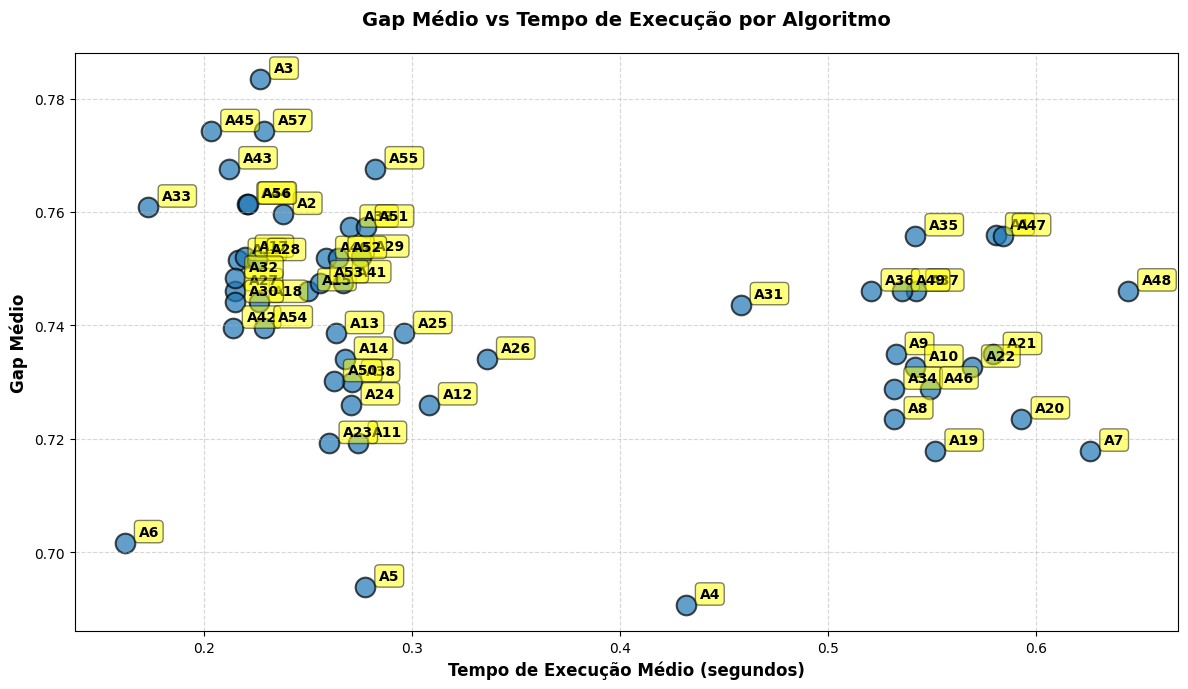
\includegraphics[width=0.92\textwidth]{Fig/simple_gap_vs_exec_time.png}
    \end{center}
\end{frame}

\begin{frame}{Seleção de Corredores}
    \begin{center}
        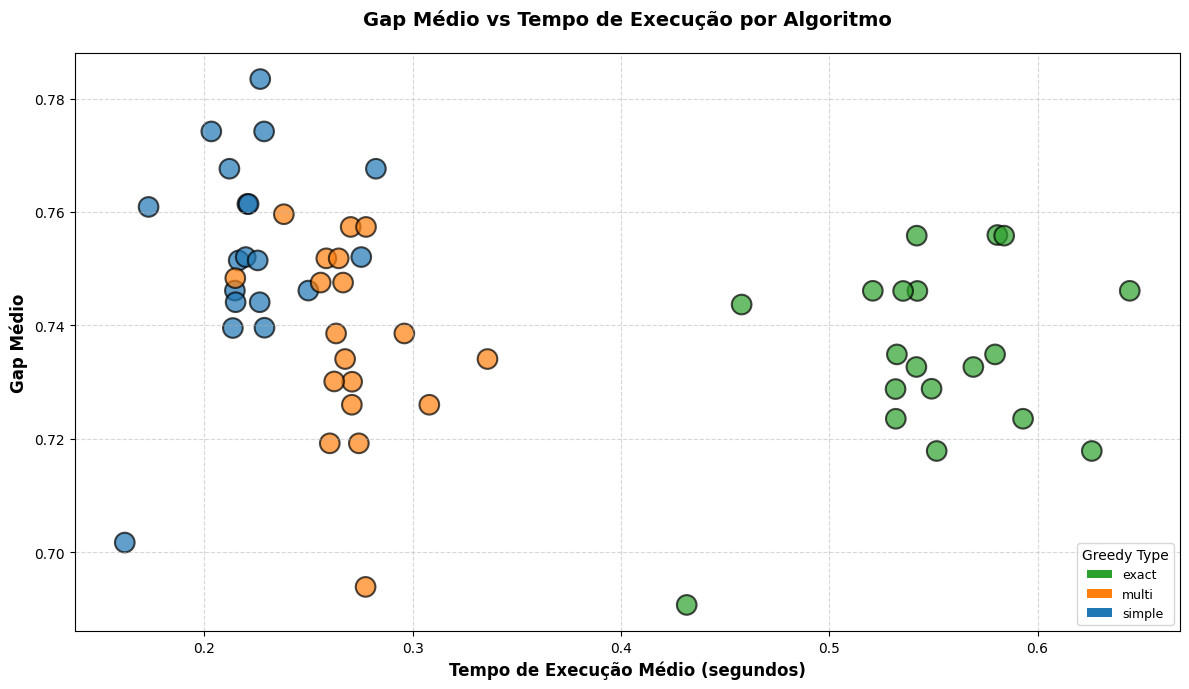
\includegraphics[width=0.92\textwidth]{Fig/gap_greedy_type.png}
    \end{center}
\end{frame}

\begin{frame}{Ordenação de Pedidos}
    \begin{center}
        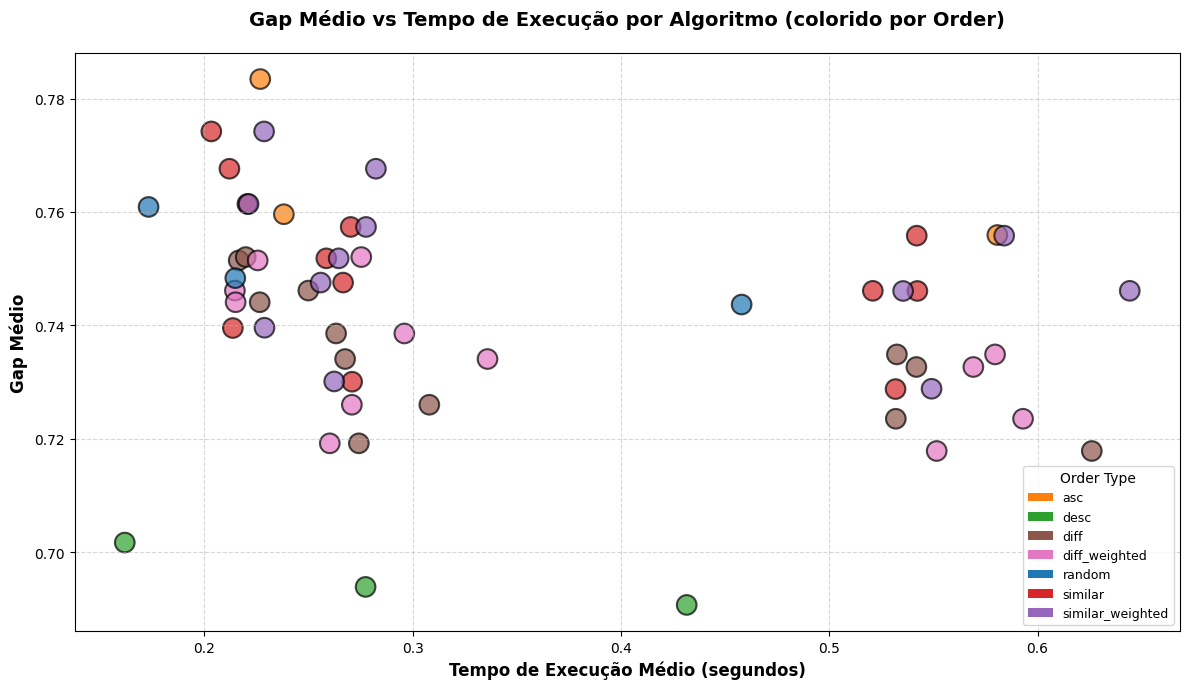
\includegraphics[width=0.92\textwidth]{Fig/gap_order_type.png}
    \end{center}
\end{frame}

\begin{frame}{Fronteira de Pareto}
    \begin{center}
        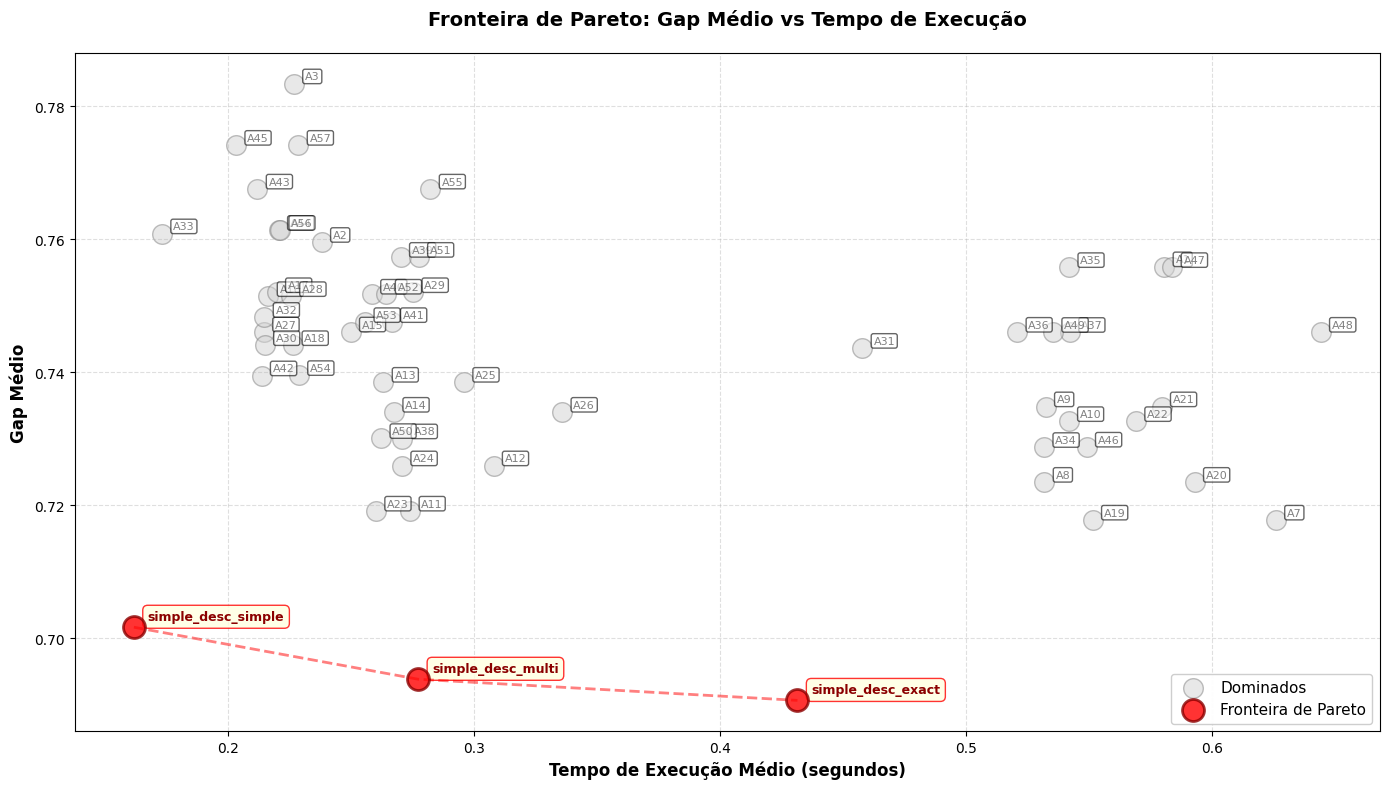
\includegraphics[width=0.88\textwidth]{Fig/simple_pareto.png}
    \end{center}
\end{frame}

% ============================================================
\section{Discussão}
% ============================================================

\begin{frame}{Discussão dos Resultados}

    \begin{itemize}
        \item
    \end{itemize}
\end{frame}

% ============================================================
\section{Conclusão e Próximos Passos}
% ============================================================

\begin{frame}{Conclusão — PFC I}
    \small
    \textbf{Objetivos cumpridos integralmente:}
    \begin{enumerate}
        \item Formalização do PSP e enquadramento na literatura do OBP
        \item Implementação da heurística gulosa com \textbf{57 variações}
              (7 critérios $\times$ 3 estratégias de corredores)
        \item Identificação das configurações Pareto-ótimas:
              \textbf{A4, A5 e A6}
    \end{enumerate}

    \bigskip
    \begin{block}{Resultado central}
        A ordenação decrescente (\texttt{desc}) é o fator dominante
        na qualidade. A estratégia de corredores opera um
        \textbf{\textit{trade-off} controlável}: de A6 (rápido) a
        A4 (melhor qualidade), todos não dominados pela fronteira
        de Pareto.
    \end{block}
\end{frame}

\begin{frame}{Próximos Passos}
    \begin{enumerate}
        \item Heurísticas por seleção de corredores
        \item Meta-heurísticas
        \item Fase 2 — Datasets B e X com análise estatística
    \end{enumerate}
\end{frame}

% ---- Agradecimentos ----
\begin{frame}[plain]
    \begin{center}
        \vfill
        Avaliação Experimental de Heurísticas e Meta-Heurísticas para o Problema Fracionário de Seleção de Pedidos Ótima
        \vfill
        \normalsize
        \textbf{Vinicius Alves Pereira} \\[0.3cm]
        \small
        Orientador: Prof.\ Ms.\ Eduardo Gabriel Reis Miranda \\
        Coorientador: Prof.\ Dr.\ André Luiz Maravilha Silva \\[0.5cm]
        Centro Federal de Educação Tecnológica de Minas Gerais \\
        Campus Divinópolis 2026
        \vfill
    \end{center}
\end{frame}

\end{document}